 %%
%% Beuth Hochschule für Technik --  Abschlussarbeit
%%
%% Hauptdokument
%%
%% 23.01.09 Tschirley V.01
%%
%%%%%%%%%%%%%%%%%%%%%%%%%%%%%%%%%%%%%%%%%%%%%%%%%%%%%%%%%%%%%%%%%%%%%
\documentclass[11pt, a4paper]{book}
%% Übersetzen als Entwurf
%\usepackage[entwurf]{bhtThesis}
%% Übersetzen für die Abgabe
\usepackage[abgabe]{bhtThesis}
\usepackage[font=small,labelfont=bf]{caption}
\usepackage{mathtools}
\usepackage{multirow,tabularx}
\usepackage{graphicx}
\graphicspath{ {./img/} }
\typeout{BHT-Abschlussarbeit V.02 15.02.12 S.Tschirley}

\usepackage{biblatex}

\usepackage{lstbayes}
\usepackage{algorithmic}
\usepackage[ruled]{algorithm2e}
\setlength\algotitleheightrule{0pt}
\SetAlgoCaptionLayout{centerline}

\makeatletter
\newenvironment{Ualgorithm}[1][htpb]{\def\@algocf@post@ruled{\kern\interspacealgoruled\hrule  height\algoheightrule\kern3pt\relax}%
\def\@algocf@capt@ruled{under}%
\setlength\algotitleheightrule{0pt}%
\SetAlgoCaptionLayout{centerline}%
\begin{algorithm}[#1]}
{\end{algorithm}}
\makeatother




\usepackage{subcaption}
\usepackage{afterpage} 
\usepackage{longtable} 
\usepackage{makecell}
\usepackage{caption}
\captionsetup[algorithm]{singlelinecheck=false}
\usepackage{pbox}
\usepackage{booktabs}
\usepackage{blindtext}   %für Blindtext in Kapitel 2
\usepackage{listings}
\usepackage{amssymb}
\usepackage{amsmath}
\usepackage{ dsfont }
\usepackage{ mathrsfs }
\usepackage{svg}

\usepackage{url}

\usepackage{color}
\definecolor{dkgreen}{rgb}{0,0.6,0}
\definecolor{gray}{rgb}{0.5,0.5,0.5}
\definecolor{mauve}{rgb}{0.58,0,0.82}


\usepackage[none]{hyphenat}
%\hyphenchar\font=-1
\sloppy

\lstset{ %
  language=R,                     % the language of the code
  basicstyle=\footnotesize,       % the size of the fonts that are used for the code
  numbers=left,                   % where to put the line-numbers
  numberstyle=\tiny\color{gray},  % the style that is used for the line-numbers
  stepnumber=1,                   % the step between two line-numbers. If it's 1, each line
                                  % will be numbered
  numbersep=5pt,                  % how far the line-numbers are from the code
  backgroundcolor=\color{white},  % choose the background color. You must add \usepackage{color}
  showspaces=false,               % show spaces adding particular underscores
  showstringspaces=false,         % underline spaces within strings
  showtabs=false,                 % show tabs within strings adding particular underscores
  frame=single,                   % adds a frame around the code
  rulecolor=\color{black},        % if not set, the frame-color may be changed on line-breaks within not-black text (e.g. commens (green here))
  tabsize=2,                      % sets default tabsize to 2 spaces
  captionpos=t,                   % sets the caption-position to bottom
  breaklines=true,                % sets automatic line breaking
  breakatwhitespace=false,        % sets if automatic breaks should only happen at whitespace
  title=\lstname,                 % show the filename of files included with \lstinputlisting;
                                  % also try caption instead of title
  keywordstyle=\color{blue},      % keyword style
  commentstyle=\color{dkgreen},   % comment style
  stringstyle=\color{mauve},      % string literal style
  morekeywords={*,...}            % if you want to add more keywords to the set
} 




%%\usepackage{hyperref}

%\usepackage[round]{natbib}

%%
%% Es folgen einige Zusätze, die in Kapitel 1 beschriben sind. 
%% Alles was nicht notwendig ist, kann auskommentiert werden
%%
\usepackage{trsym}
%\usepackage{showkeys}
\usepackage{bytefield}

\def\blankpage{%
      \clearpage%
      \thispagestyle{empty}%
      \addtocounter{page}{-1}%
      \null%
      \clearpage}

%%
%% Pfad zu den Bildern
%%
\graphicspath{
  {img/},
}

%%
%% Einbinden persönlicher macros 
%%
%
% Persönliche Macros
%
%

% Macros für Formeln
\newcommand{\jw}{j\omega}

% Begriffe

\newcommand{\OPV}{Operations\-ver\-stär\-ker}



%% Message
\typeout{-----------------------------------------------------------}
\typeout{----> main.tex ---- Zentrales Dokument---------------------}
\typeout{-----------------------------------------------------------}

\version{0.1$\alpha$}
\datum{\today}
%%
%% Titel, Autor und Betreuer
%%
\fachbereich{VI} 
\studiengang{Medieninformatik}
\autor{Sebastian Herrmann}
\edvnr{852049}
\titel{Generating Electronic Medical Records}
%\untertitel{Evaluating the Accuracy of Variational Bayes Variational Inference in Survival Analysis}
\betreuerFeld{
  \begin{tabular}{lr}
    \multicolumn{2}{l}{\textbf{Gutachter}}\\
    Prof. Dr.-Ing. habil. Alexander Löser & Beuth Hochschule für Technik Berlin\\
    Prof. Dr. Felix Bießmann & Beuth Hochschule für Technik Berlin
  \end{tabular}
}

%%%%%%%%%%%%%%%%%%%%%%%%%%%%%%%%%%%%%%%%%%%%%%%%%%%%%%%%%%%%%%%
%% Literaturverzeichnis

\clearpage\newpage
\addcontentsline{toc}{chapter}{References}
%\bibliographystyle{myapalike}
\bibliographystyle{apa}
\bibliography{library}
\

%%\renewcommand{\baselinestretch}{1.05} 
\begin{document}
\pagestyle{fancy}
\thispagestyle{empty}
\renewcommand{\bibname}{References}

%makecell package formatting
\renewcommand\theadfont{\normalsize}
%\renewcommand\theadfont{\itshape}

\thispagestyle{empty}
\maketitle

\blankpage

\thispagestyle{empty}
\section*{Abstract}
XXX


\blankpage

\clearpage

\thispagestyle{empty}
\tableofcontents

\blankpage


\pagenumbering{arabic}
%%%%%%%%%%%%%%%%%%%%%%%%%%%%%%%%%%%%%%%%%%%%%%%%%%%%%%%%%%%%%%%





\chapter{Introduction (total approx. 5 pages)}
% Am Anfang jedes Kapitels kurze Übersicht, was das Kapitel beinhaltet

\section{Problem}
\section{Goal}

\section{Method}
\subsection{Preliminary: GAN}
TODO
\subsection{medGAN}
TODO
\subsection{binary/count variables}
For our experiments, we generated both, records with binary and count variables. Records with binary data will show whether an ICD code occured or not, while records with count data will show how many times each ICD code occurred for each patient.
\subsection{privacy risk}
As the synthetic data is artificially created, there is no direct connection between the real and the synthetic samples. Therefore identifying patients from the original dataset should, intuitively, not be possible with the help of the artificially created samples.  To assess the privacy risk, \cite{Choi2017}
\section{Overview}

\chapter{Related Work (approx. 5-8 pages)}
\section{Abstract}
The following section will elaborate the basic concepts that are needed to  generate synthetic electronic health record data.
First, we explain the concept of a Generative Adversarial Network. Further we will define what exactly an Electronic Health record is. Subsequently we will introduce the definition of Gender Medicine.

\section{Basic Concepts}
\subsection{Generative Adversarial Networks}
This section will explain the concept of Generative Adversarial Networks and their role for this work.
In \cite{goodfellow2014generative} proposed a new framework for generative models, that learns the patterns in the data and generates new data that plausibly could originate from the original dataset.
 The model corresponds to a two-player minimax game in which two independent neural networks train simultaneously: a generator \textbf{G} which is learning the distribution of the given data and a discriminator \textbf{D} which aims to distinguish between the data from the training set and from \textbf{G}.

In this game, G has the goal to maximize the probability of D making a mistake.  \cite{goodfellow2014generative}
\\
\\
The two-player minimax game can be described by the following value function:
\\
\begin{equation}
	\min_G\max_DV(D,G) = \mathbb{E}_{x\sim{P_{data(x)}}}[log D(x)] + \mathbb{E}_{z\sim_{P_z(z)}}[log(1 - D(G(z)))]
\end{equation}
\cite
\\

For better understanding of the process of the model, the analogy can be helpful:
"The generative model can be thought of as analogous to a team of counterfeiters, trying  to  produce  fake  currency  and  use  it  without  detection,  while  the  discriminative  model  is analogous to the police, trying to detect the counterfeit currency.  Competition in this game drives both teams to improve their methods until the counterfeits are indistinguishable from the genuine articles." \cite{goodfellow2014generative}

% minGmaxDV(D,G) =Ex∼pdata(x)[logD(x)] +Ez∼pz(z)[log(1−D(G(z)))].
\subsection{Electronic Health Records}
"The Electronic Health Record (EHR) is a longitudinal electronic record of patient health information generated by one or more encounters in any care delivery setting. Included in this information are patient demographics, progress notes, problems, medications, vital signs, past medical history, immunizations, laboratory data and radiology reports." \cite{HIMMS}
%eo
\subsection{Gender Medicine}
Medical research is dominated by the male gender, meaning that women are heavily underrepresented or sometimes even excluded from research studies not only in animal studies but also in human trials. \cite{baggio2013gender} 
But "diseases  differ  between  men  and  women  in  terms  of  prevention,  clinical  signs,  therapeutic  approach,  prognosis,  psychological  and  social  impact." \cite{baggio2013gender}
Sex-differences can also be found in the correlation of diseases. \cite{kautzky2010sex} shows in his research, that "Sex-specific differences appear particularly relevant in the management of type 2 diabetes mellitus (T2DM), with women experiencing greater increases in cardiovascular morbidity and mortality than do men." \cite{kautzky2010sex}
Gender however does not only include sex, but also lifestyle-related diseases, stress and behaviour, like for example regarding help-seeking actions.
While we can not take the socio-cultural aspect of gender into account, the differences in sex are applicable.
As "cardiovascular disease is the leading cause of death of both men and women" \cite{arain2009sex}, we can find numerous occurrences in the MIMIC-III dataset. This allows us to investigate co-occurrences of diabetes and CVD.
Originally MedGAN was trained with male and female patients simultaneously, making no difference between them. In this work we are separating the dataset in order to introduce a distinction between genders.

The previously mentioned gender-differences lead us to one of our hypotheses, that will be formulated in Chapter 4.

\subsection{medGAN}
The wide adoption of the electronic health record system by healthcare organizations (HCOs) promises advances in analyzing patient data and computational health. The records however are not easily accessible for researchers. Due to the fact that EHR data consists of personal and sensitive information, access is restricted in order to not induce a privacy risk. Further, to minimize the risk of data misuse, access to such data is regulated by the HCOs. \citep{Choi2017}
(Even researches that are in a direct cooperation with a hospital, do not get access to patient data.)
 As \cite{Choi2017} states, "[t]he review process by legal departments and institutional review boards can take months, with no guarantee of access (Hodge Jr et al., 1999). This process limits timely opportunities to use data and may slow advances in biomedical knowledge and patient care (Gostin et al., 2009)."
 \cite{Choi2017} describes, that "HCOs often aim to mitigate privacy risks through the practice of de-identification (for Civil Rights, 2013), typically through the perturbation of potentially identifiable attributes (e.g., dates of birth) via generalization, suppression or randomization. (El Emam et al., 2015) However, this approach is not impregnable to attacks, such as linkage via residual information to re-identify the individuals to whom the data corresponds (El Emam et al., 2011b). An alternative approach to de-identification is to generate synthetic data (McLachlan et al., 2016; Buczak et al., 2010; Lombardo and Moniz, 2008). However, realizing this goal in practice has been challenging because the resulting synthetic data are often not sufficiently realistic for machine learning tasks."  \cite{Choi2017}
 To overcome the limitations and risks of the above stated methods, \cite{Choi2017} introduced medGAN, which implements a Generative Adversarial Network that leverages an autoencoder to overcome its limitations: the GAN generates distributed representations of patient records, while the autoencoder decodes them into actual discrete records.
 This principle and the detailed architecture of medGAN will be further explained in the section 'Electronic Medical Record Generation'.

\section{Summary}

\chapter{Data Analysis}
Before conducting our research we performed an exploratory data analysis on the MIMICIII dataset. The goal of this analysis was to discover patterns and correlations in the data to formulate hypotheses for further analysis. "MIMIC-III [2] is a freely accessible dataset developed by the MIT lab for computational physiology utilized by numerous researchers and scholars world wide. The database consists of demographics, vital signs, laboratory tests, medications, caregiver notes, and mortality of approximately 40,000 intensive care unit patients at Beth Israel Deaconess Medical center between 2001 and 2012." \cite{arya2019exploratory}
We used pandas and numpy for the analysis and matplotlib, to display the results.

The following section will display the results...

The total number of unique patients found in the dataset is 46260, consisting of 26121 male of 20399 female patients.

\begin{figure}
  \begin{center}
  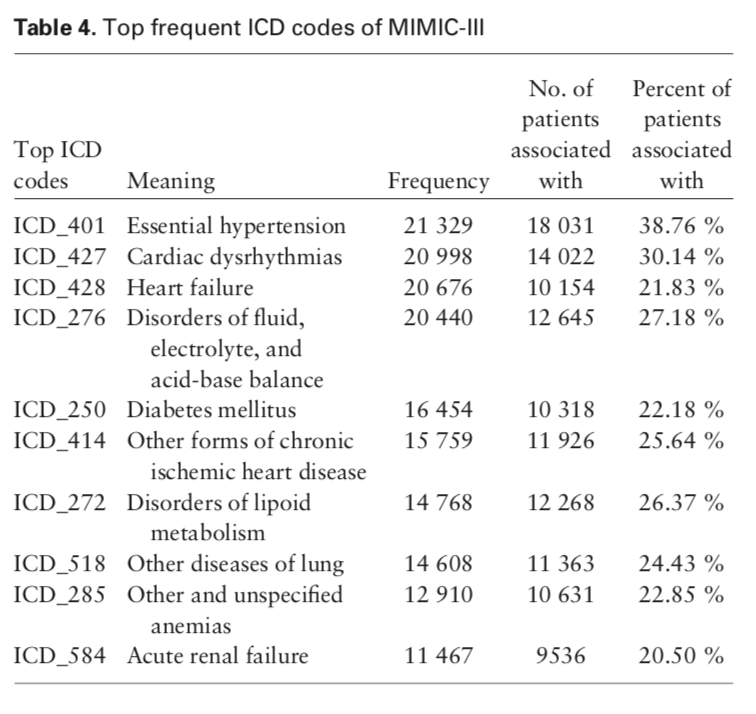
\includegraphics[width=0.5\textwidth]{icd_top_frequency}
  \caption{The traditional supervised learning setup in machine learning. \cite{Ruder2019}}
  \label{fig:transfer_learning_no}
  \end{center}
\end{figure}

\begin{figure}
  \begin{center}
  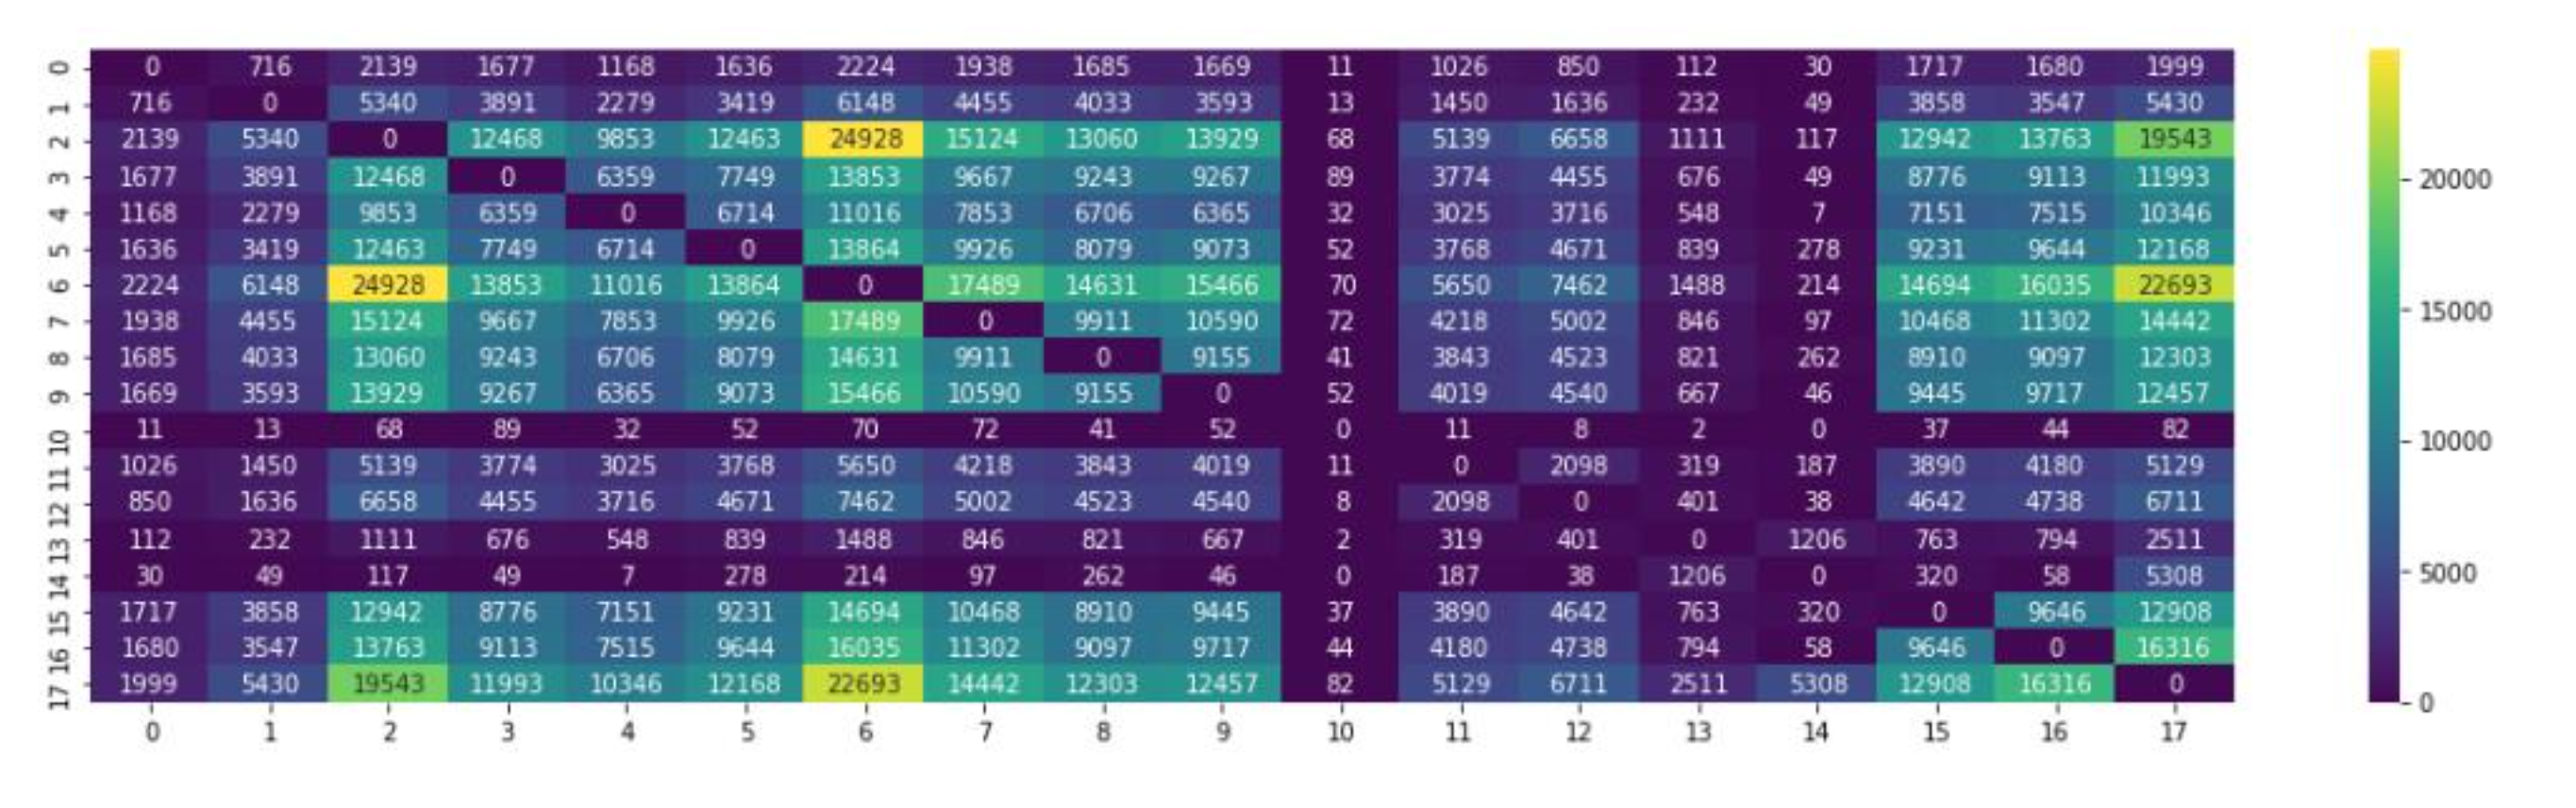
\includegraphics[width=0.5\textwidth]{img/correlation-heatmap.png}
  \caption{The traditional supervised learning setup in machine learning. \citep{Ruder2019}}
  \label{fig:transfer_learning_no}
  \end{center}
\end{figure}

The correlation heatmap that is introduced in \cite{arya2019exploratory}
shows the strongest correlation of ICD9 codes from the groups two and six which correspond to endocrine, nutritional and metabolic diseases and immunity disorders and diseases of the circulatory system.

We further investigated  these groups and focus on comparing the cooccurrence of ischemic and diabetic diseases. 

First, we compare the top 12 occcurences of male and female diagnoses of heart disease

\begin{figure}
  \begin{center}
  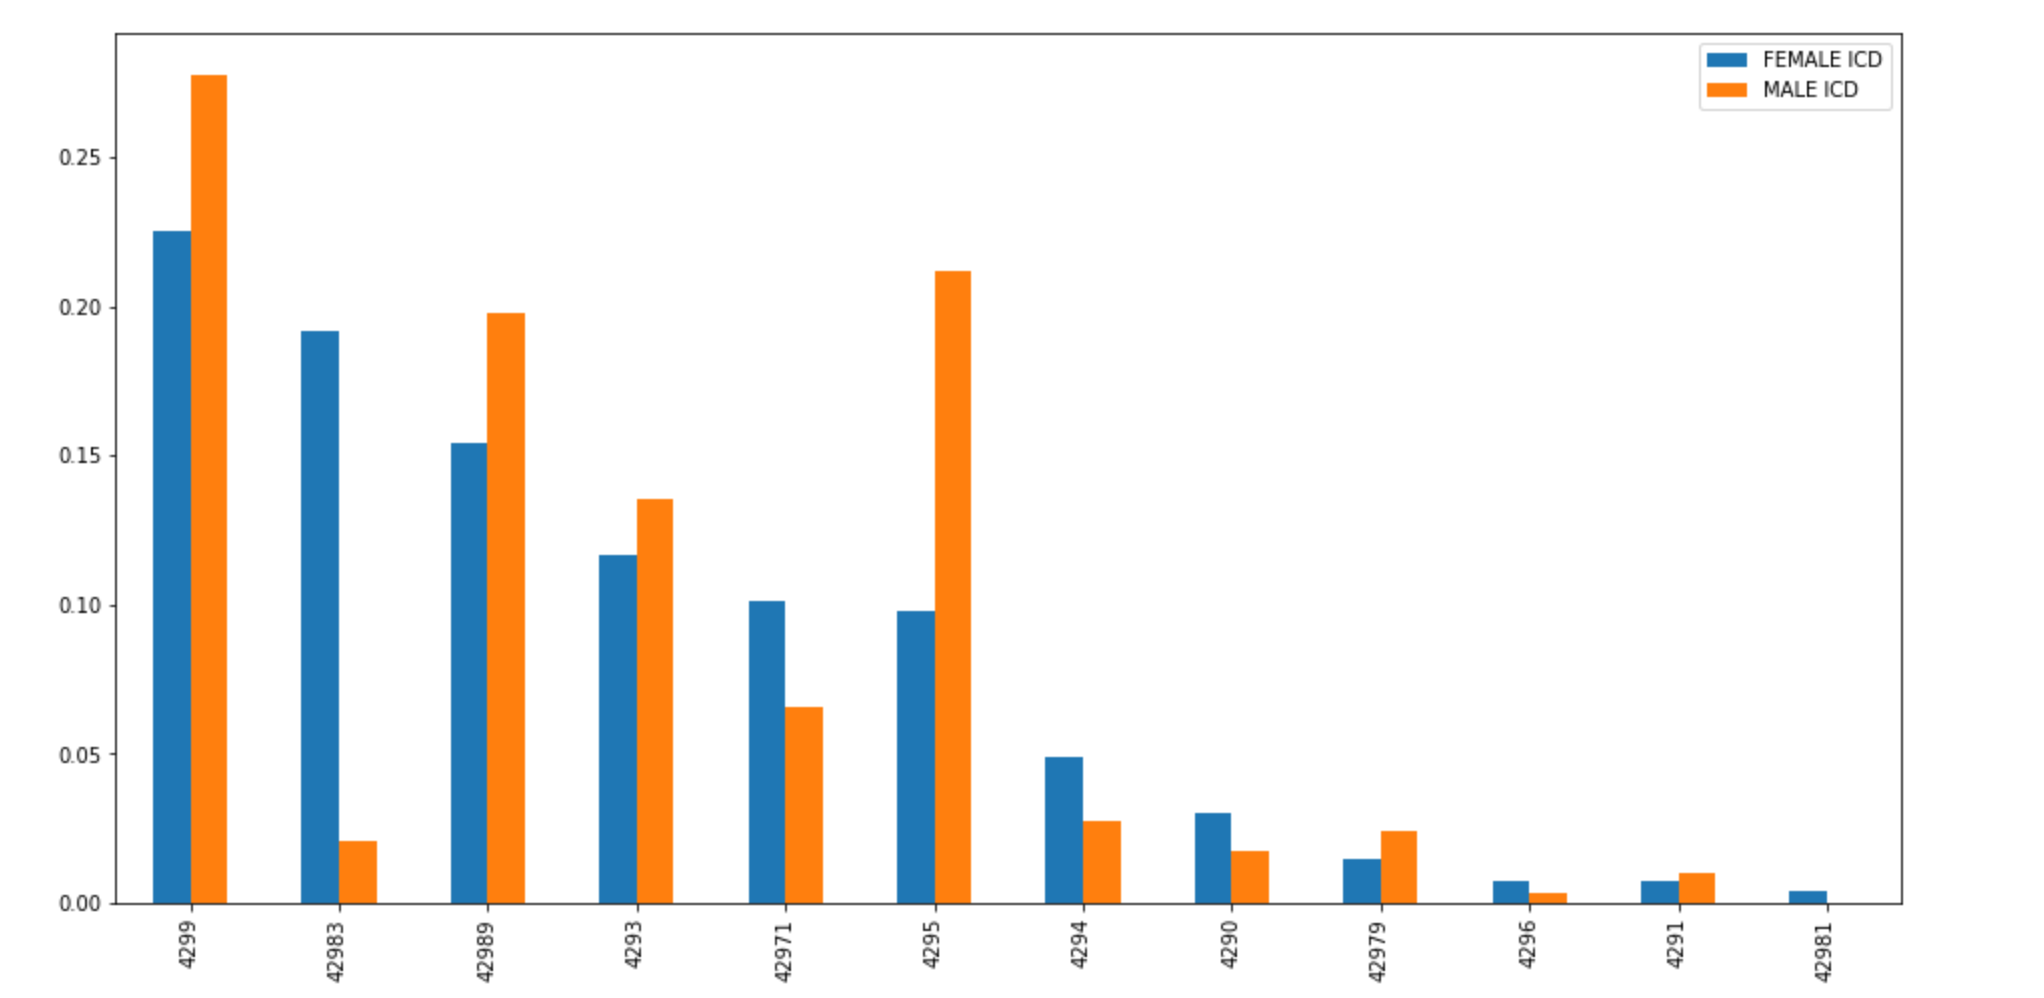
\includegraphics[width=0.5\textwidth]{img/male_female_heart_disease.png}
  \caption{Comparison male/female heart disease. The X axis describes the ICD9 code, the Y axis the percentage of affected patients.}
  \label{fig:heart_disease_comparison}
  \end{center}
\end{figure}

Out of 46260 patients, in our dataset 14851 female and 19185 male are diagnosed with any form of heart disease. We can see, that mostly women are affected by Takotsubo syndrome (ICD9-Code 429.9) and that around twice as many men are affected by Rupture of chordae tendineae as women (ICD9-Code 429.5). For unspecified Heart diseases (code 429.9) and other ill-defined heart diseases (code 429.89) more men are affected.  However we can find more women affected by functional disturbances following cardiac surgery and unspecified Myocarditis. 

Second, we compare males and females diagnosed with diabetic diseases: (ICD9 250.*). 7280 females and 9174 males are affected.

\begin{figure}
  \begin{center}
  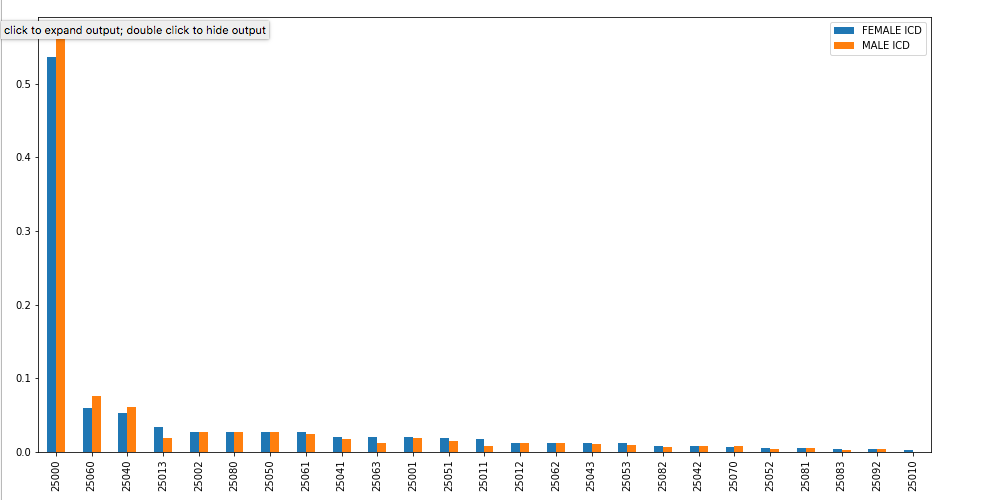
\includegraphics[width=0.5\textwidth]{img/comparison_diabetic.png}
  \caption{Comparison male/female diabetic disease. The X axis describes the ICD9 code, the Y axis the percentage of affected patients.}
  \label{fig:diabetic_comparison}
  \end{center}
\end{figure}

As explained in [Basic concepts - Gender medicine] correlations between diabetes and heart disease find their cause in this subject

\chapter{Electronic Medical Record Generation (approx. 15 pages}
\section{Abstract}
In this chapter, we will elaborate medGAN, discuss the process and architecture, our experimental setup and the process of training and generating synthetic Electronic Medical Record data. Further, we will introduce our hypotheses and describe the dataset.
\section{medGAN}
D and G are both implemented as feedforward neural networks.
As we learned in (SECTION GAN), the generator G "is trained by the error signal from the discriminator D via backpropagation, the original GAN can only learn to approximate discrete patient records x ∈ Z|C| with continuous values. ” \citep{Choi2017}

To alleviate this limitation, they leveraged an autoencoder which is reconstructing an dimensionality reduced approximate of the input. As \cite{Choi2017} stated, “[s]uch a mechanism leads the autoencoder to learn salient features of the samples and has been successfully used in certain applications, such as image processing (Goodfellow et al., 2016; Vincent et al., 2008).” 

The objective of the autoencoder is, to minimize the reconstruction error:

FORMEL AUTOENCODE
\begin{equation}
\frac{1}{m}\big[\sum_{i=0}^m \mid\mid x_i - x_i`\mid\mid_2^2]
\end{equation}
\begin{equation}
\frac{1}{m}\big[\sum_{i=0}^m x_i \log x´_i + (1-x_i) \log (1-x´_i)]
\end{equation}

FORMELN STIMMEN NOCH NICHT
where m is the size of the mini-batch.


An autoenconder consists of of two elements: The Encoder (Enc) which compresses the input and the Decoder (Dec) that is used to construct the output.
For count variables they used the cross entropy loss and rectified linear units  as activation function for the Enc and Dec.
For binary variables they used the mean squared loss and the tanh activation function for Enc and the sigmoid activation for Dec.
Both, the Enc and the Dec are implemented as single layer feedforward networks. The original input x it receives, is compressed into a 128 dimensional vector. The generator G consists of two hidden-layers with each 128 dimensions and is implemented as a feedforward network. For the batch normalization in G they use the scale parameter  \gamma and the shift parameter \beta and set the moving average decay to 0.99. The discriminator D has the same structure, but the first hidden-layer consists of 256 dimensions. medGAN is trained for 1,000 epochs with the mini-batch of 1000 records. \cite{Choi2017}


\begin{figure}
  \begin{center}
  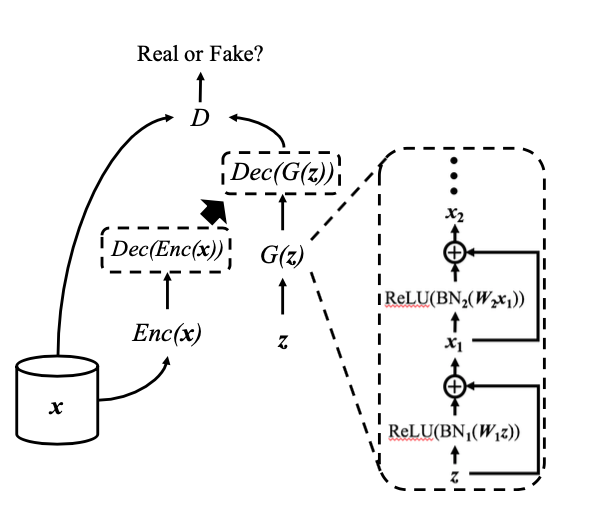
\includegraphics[width=0.5\textwidth]{img/medgan-architecture.png}
  \caption{Architecture of medGAN: The discrete x comes from the source EHR data, z is the random prior for the generator G; G is a feedforward network with shortcut connections (right-hand side figure); An autoencoder (i.e, the encoder Enc and decoder Dec) is learned from x; The same decoder Dec is used after the generator G to construct the discrete output. The discriminator D tries to differentiate real input x and discrete synthetic output Dec(G(z)).  \citep{Choi2017}}
  \label{fig:transfer_learning_no}
  \end{center}
\end{figure}

"medGAN generates synthetic EHR datasets that achieve comparable performance to real data on many experiments including distribution statistics, predictive modeling tasks and medical expert review."

UMFORMULIEREN (zitiert)

\subsection{SynthEHR (medBGAN, medWGAN)}
In \citep{Baowaly2018} proposed two altered versions of medGAN that outperform their predecessor, however just slightly.
Those two versions are:

\textbf{medWGAN}: This version substitutes the regular GAN with an improved \textit{Wasserstein GAN (WGAN)}, that utilizes "an alternative method of weight clipping called gradient penalty, which entails penalizing the norm of the gradient of the discriminator (critic) with respect to its input" \citep{Baowaly2018}

\textbf{medBGAN}: This version substitutes the regular GAN as well, but this time with a \textit{boundary-seeking GAN (BGAN)}. This approach trains the generator to match the target distribution that converges toward the true distribution as the discriminator is optimized" \citep{Baowaly2018}
\subsection{Differentiation}
Bereits erklärt?
\subsection{Why left out?}
If our hypotheses proof to be true and bring an improvement to medGAN, these improvements will also translate to altered versions of medGAN, because not the network itself is being changed but the input. In our tests we separated the dataset and did not alter it. Henceforth we performed our tests only on the 'original' medGAN. 
\section{Process and Architecture}
For generating the Electronic Medical Records (EMR), we used a Generative Adversarial Network (GAN) called medGAN, that was proposed in \citep{Choi2017}. As input data we use v1.4 of the MIMIC-III (Medical Information Mart for Intensive Care) dataset. For our experiments, we divided the dataset by gender and generated EMR data with binary and count variables for both mixed and separated patients. The code for medGAN is publicly accessible under https://github.com/mp2893/medgan. It is implemented using TensorFlow
For training models, they chose the Adam-optimizer with a mini-batch size of 100 patients. \citep{Choi2017} We trained the model using Colaboratory by Google, which is a Jupyter notebook environment, providing free Cloud computing for education and research.
The machines are equipped with K80 GPUs from NVIDIA.
With the K80 GPU, it took 29 minutes and 3 seconds to train the model with only female patients, 35 minutes and 26 seconds to train the model with only male patients and 60 minutes and 1 second to train the model with the full dataset.
\section{Experimental Setup}
 For training, we split the data into subsets with a ratio of 9:1 for training and validation subsets. Using the training subset, the autoencoder is pretrained for 100 epochs. 
 After each epoch, we report the training and validation loss. For binary variables we use the cross-entropy loss  function, for count variables the mean squared error.
 Further, we use minibatch averaging and batch normalization
We conducted our data analysis in a Jupyter Notebook. Here, we use pandas to investigate the data and matplotlib to show our results.
After finishing the training process, we select the epoch closest to 0.5, since that is when the discriminator is most confused and the generator makes the most convincing synthetic samples.


\section{Hypothesis}
In this work we are trying to proof the following three hypotheses:

First, the model can generate realistic patients if it is trained with the MIMIC III dataset / the model learns the distribution of ICD9 codes.
Second, by training the network with female and male patients separately, it is able to generate patients with gender-specific correlated diseases that seem realistic to a medical doctor.
Third, if the network is being trained with the MIMIC-III dataset, it is able to generate patients affected by orphan diseases that can not be distinguished to a non-synthetic patient by a medical doctor



\section{Data}
The dataset is publicly available for researchers worldwide. In order to gain access to it we were required to complete the CITI “Data or Specimens Only Research” course.

It contains deidentified health-related data associated of over forty thousand patients who stayed in critical care units of the Beth Israel Deaconess Medical Center in Boston between 2001 and 2012.

We extracted the ICD9 codes for female and male patients from the dataset separately and aggregated a patient’s longitudinal record into a single fixed-size vector  x elem Z{$^C$}. For ICD9-Codes shortened to 3 digits, $C$ equals 1071 for mixed patients, 987 for female patients and 966 for male patients. For, full-length 5 digits ICD9-Codes $C$ equals 6985 for mixed patients, 5650 for female patients and 5853 for male patients.

TODO: GLEICHUNGEN

Model for comparison: 

To assess the effectiveness of my method, I trained the network both, with mixed and gender-separated patients. 

\cite{Choi2017} also compared medGAN with other popular generative methods like Random Noise, Independent Sampling. In his experiments, medGAN outperformed other methods. Therefore we will compare our results with medGAN.

\section{Models for Comparison}
For our baseline we choose medGAN as proposed in \cite{Choi2017}. As stated in the paper, medGAN outperformed machine learning models like Linear Regression and Random Forests
\section{Measurements}
For comparison we generated samples of sizes, equal to the dataset.

\section{Summary}

\section{Non-Gender-specific EMR Generation}
First, like in \citep{Choi2017} we generated EMR data, without dividing the dataset. The results serve as baseline for the performance and will be compared with the separately generated patients.
\\
\\



\section{Gender-specific EMR Generation}
Second, we divided our dataset by gender and generated patient data separately, resulting in 20399 female and 26121 male unique records.
\\
%\section{Rare diseases}
Wikidata provides a mapping of 4584 ICD-9 codes to GARD and OrphaNet IDs.
To investigate the occurrence of rare diseases in MIMIC-III, we first generated a list containing all 6985 unique ICD9 codes of the dataset. Then, we match the list from the mapping which contains a total of 962 codes, resulting in ten corresponding codes in the MIMIC-III dataset. 2408 diagnoses with orphan ICD9-codes are present in the given dataset.

The following section will elaborate our findings regarding rare diseases in our generated patients.
\chapter{Experimental Evaluation}
\section{Abstract}
In the following section we will, evaluate our expermiments in order to measure our success. First, in a quantitative manner, using three statistical methods. Second, by evaluation in a qualitative manner, comparing the generated data to the original dataset and with the help of a medical doctor.
\section{Hypotheses}
In our work we are trying to proof the following hypotheses:
First, we are making the assumption that the model can generate realistic patients if it is trained with the MIMIC III dataset / the model learns the distribution of ICD9 codes.
Second, by training the network with female and male patients separately, it is able to generate patients with gender-specific correlated diseases that seem realistic to a medical doctor -> improvement
- if the network is being trained with the MIMIC-III dataset, it is able to generate patients affected by orphan diseases that can not be distinguished to a non-synthetic patient by a medical doctor



\section{Measurements}
\textbf{Orphan diseases}:
\\
\\
\begin{tabularx}{\textwidth}{p{0.55\textwidth}|r|X|r}
ICD9-Code & Female Binary & Male Binary & Mixed\\
\hline
042 Human immunodeficiency virus [HIV] disease	& 739 & 144	& 121\\
515 Postinflammatory pulmonary fibrosis & 0 & 168 & 907\\
570 Acute and subacute necrosis of liver & 255	& 0	& 33\\
\end{tabularx}
\\
\\
\begin{tabularx}{\textwidth}{p{0.55\textwidth}|r|X|r}
ICD9-Code & Dataset Female & Dataset Male\\
\hline
075 Infectious mononucleosis & 7 & 4\\
138 Late effects of acute poliomyelitis & 36 & 37 \\
193 Malignant neoplasm of thyroid gland & 21 & 28 \\
220 Benign neoplasm of ovary & 25	& 0\\
317 Mild intellectual disabilities & 43 & 39\\
8832 Open wound of finger(s), with tendon involvement & 2 & 15\\ 
\end{tabularx}
	
\section{Evaluation}
\subsection{Abstract}
In this section we will evaluate our measurements in a quantitative and qualitative manner. We evaluate the measurements for 3 digit (shortened) and 5 digit (original) ICD9-codes for both, binary and count variables.
First comes the quantitative evaluation of our generated records. For this we choose two statistical methods: dimension-wise probability for binary variables and dimension-wise average for count variables.
Second we perform the qualitative evaluation. We begin with investigating the data, like we did with the real dataset, looking for correlations of diabetic-disease and heart-disease. Subsequently, we evaluate our measurements with the help of a medical doctor.
\subsection{Quantitative Evaluation UMFORMULIEREN}
For the quantitative evaluation of our measurements we choose the following statistical methods, as presented in \citep{Choi2017}.
\\
\\
\textbf{Dimension-wise probability}: This refers to the Bernoulli success probability of each dimension (disease or procedure code) in the binary dataset. The dimension-wise probability is computed using the following formula: 

\begin{equation}
Number\,of\,patients = \frac{Number\,of\,patients\, who \,had \,the \,disease}{Total \,number \,of \,patients}
\end{equation}

We calculate it for the binary data.
\\

\textbf{Dimension-wise average}: This refers to the column average of each dimension (disease or procedure code) in the count dataset. The dimension-wise average is calculated using the following formula: 
\begin{equation}
Dimension-wise\,average = \frac{Column \,sum}{Total \,number \,of \,records}
\end{equation}

We calculate it for the count data.
\\
For both, dimension-wise probability and dimension-wise average, we present the outcomes in a scatterplot. Each dot represents a diagnoses code. The x-axis represents the codes from the real data, the y-axis the one's from the synthetic data.

\textbf{Dimension-wise K–S test}: We performed the K–S test on 2 data samples (synthetic data and real data) to examine whether the 2 data samples originate from the same distribution. In the K–S test, the statistic is calculated by finding the maximum absolute value of the differences between 2 samples’ cumulative distribution functions. The null hypothesis is that both samples originate from a population with the same distribution. In our experiment, we rejected the null hypothesis with a low P-value (typically 􏰆 0.05). More details of the K–S test is discussed in the Results section. 

\begin{figure}
\centering
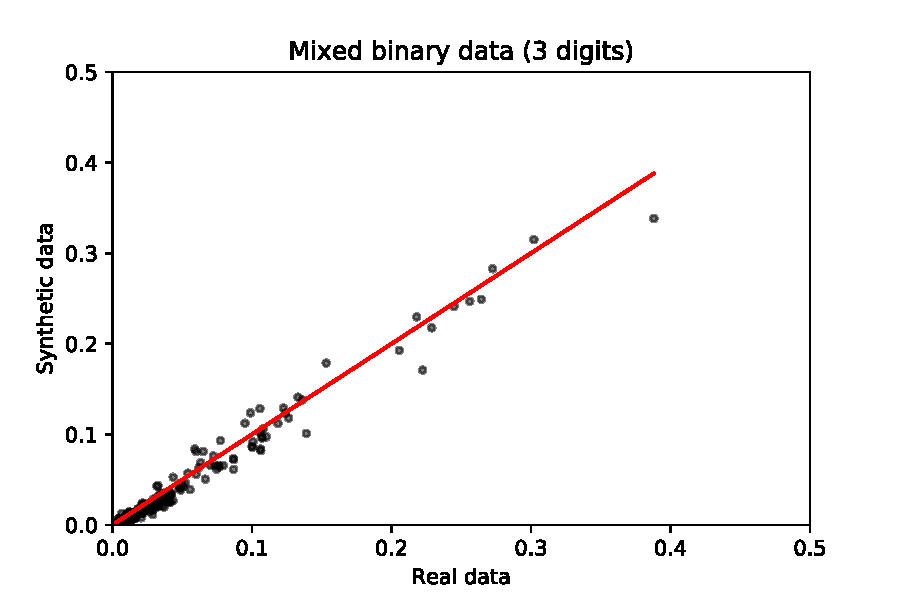
\includegraphics[width=.3\textwidth]{img/plots/binary_3digit_mixed}\hfill
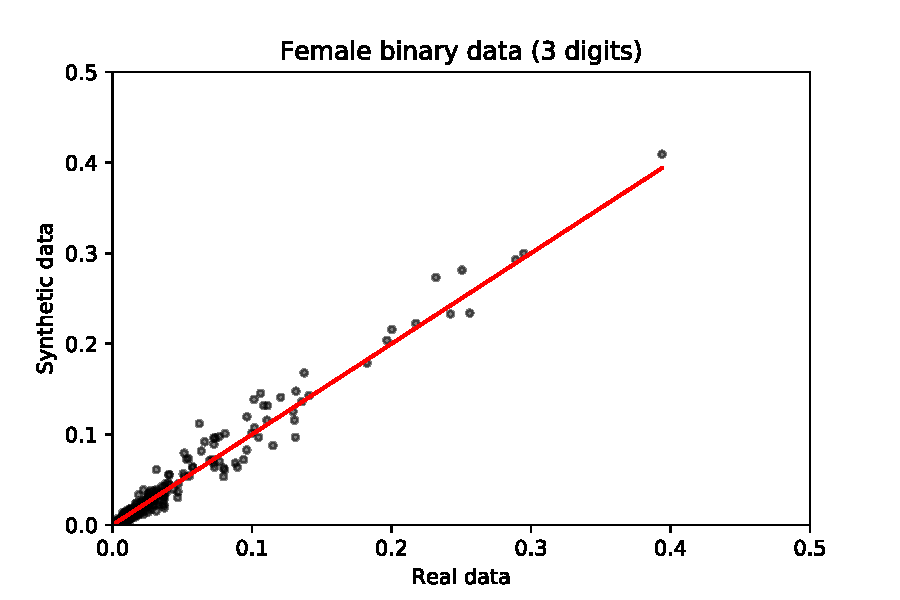
\includegraphics[width=.3\textwidth]{img/plots/binary_3digit_female}\hfill
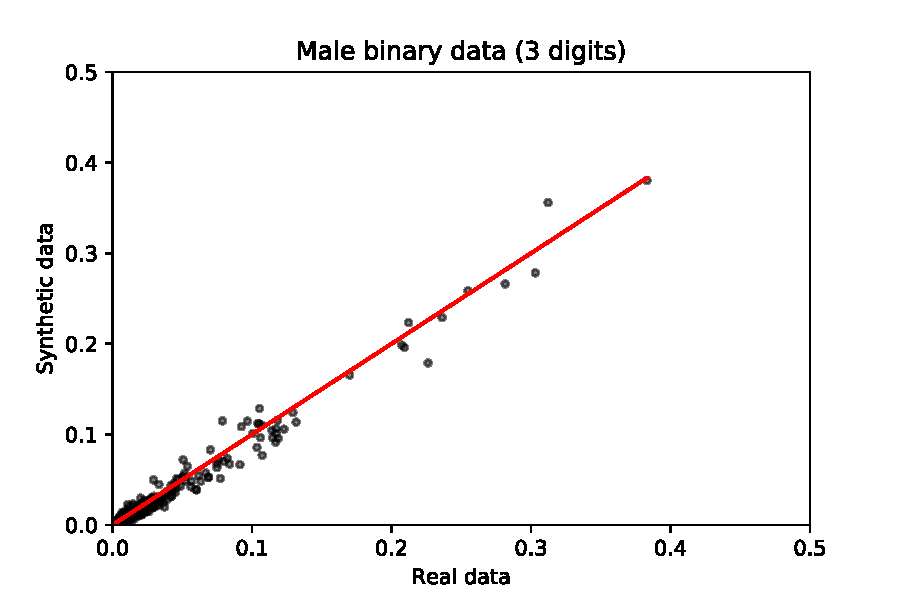
\includegraphics[width=.3\textwidth]{img/plots/binary_3digit_male}\hfill
\\
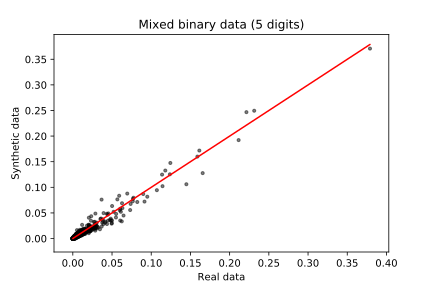
\includegraphics[width=.3\textwidth]{img/plots/binary_5digit_mixed}\hfill
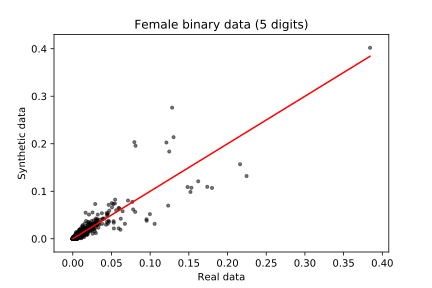
\includegraphics[width=.3\textwidth]{img/plots/binary_5digit_female}\hfill
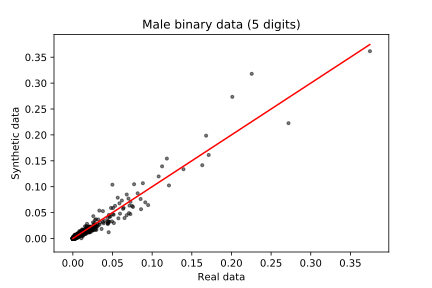
\includegraphics[width=.3\textwidth]{img/plots/binary_5digit_male}\hfill
\caption{dimension-wise probability}
\label{fig:figure3}
\end{figure}

\\
\\
\begin{figure}
\centering
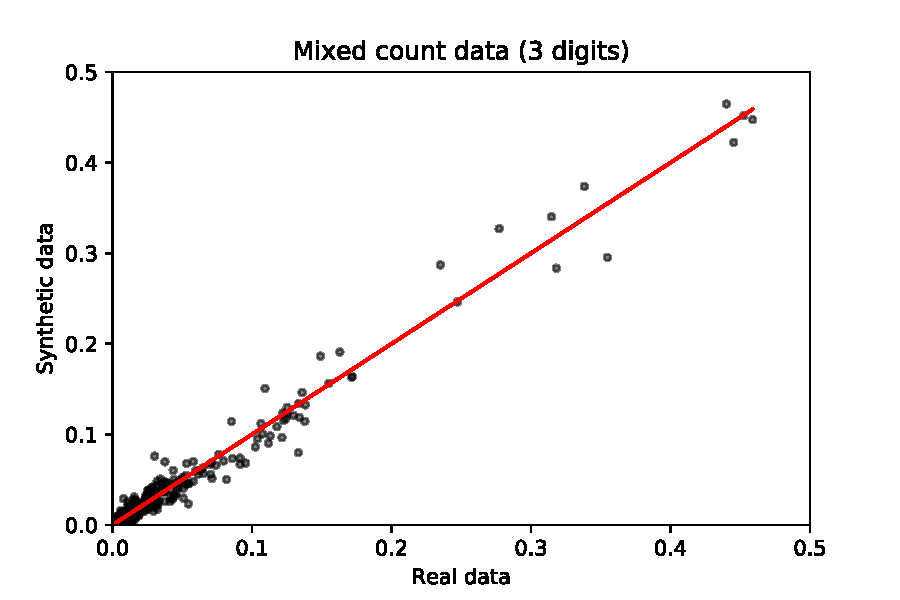
\includegraphics[width=.3\textwidth]{img/plots/count_3digit_mixed}\hfill
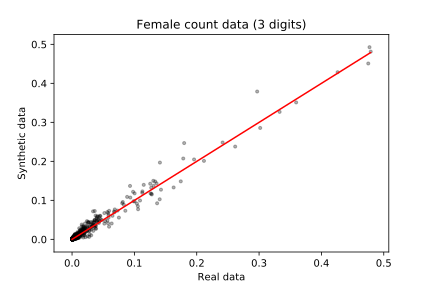
\includegraphics[width=.3\textwidth]{img/plots/count_3digit_female}\hfill
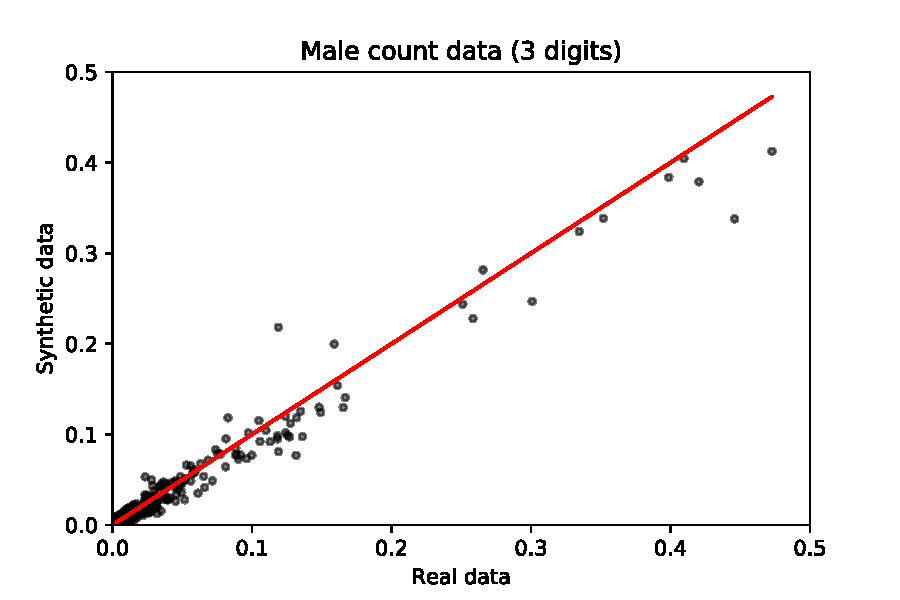
\includegraphics[width=.3\textwidth]{img/plots/count_3digit_male}\hfill
\\
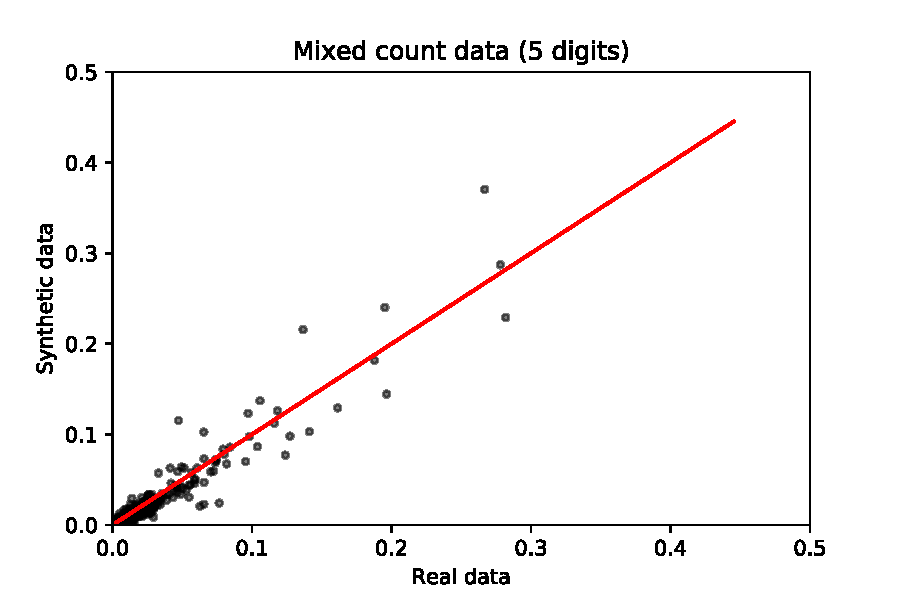
\includegraphics[width=.3\textwidth]{img/plots/count_5digit_mixed}\hfill
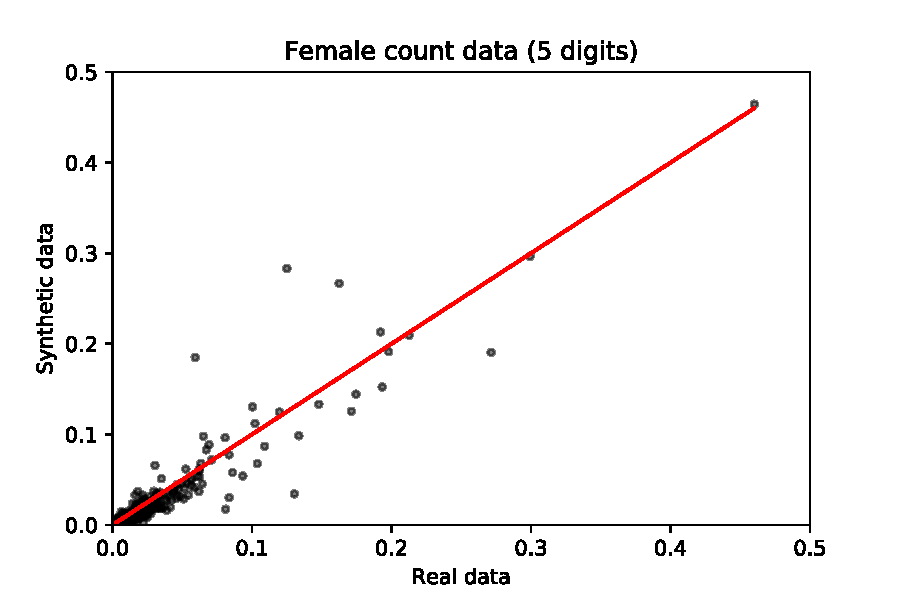
\includegraphics[width=.3\textwidth]{img/plots/count_5digit_female}\hfill
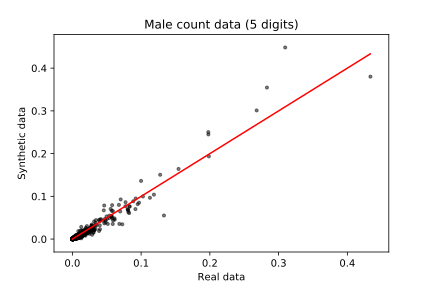
\includegraphics[width=.3\textwidth]{img/plots/count_5digit_male}\hfill
\caption{dimension-wise average}
\label{fig:figure3}
\end{figure}

\subsubsection{Evaluation Orphan diseases}


\subsection{Qualitative Evaluation}
Our qualitative evaluation consists of three parts. First, we repeat the steps of our data analysis and compare our synthetic samples with it. Second, we investigate the synthetic dataset on gender-specific correlations and rare diseases. Third, we rate our measurements with the help of a medical doctor. Therefore we take 25 samples from the original dataset and 25 samples from our generated patients. Then, we present them in random order to a medical doctor and let him rate them on realisticness on a scale from 1 to 10, where 10 is the highest score and therefore a sample, that can not be distinguished from a real record.
The samples are selected randomly, except for the rare diseases. Here we choose 5 samples each from the dataset and from our generated patients because of their scarcity.

\subsubsection{Data analysis}

\begin{table}
\begin{tabularx}{\textwidth}{p{0.55\textwidth}|r|X|r}
\textbf{ICD9-Code} & \textbf{Percent of affected patients}\\
\hline
401.9 Unspecified essential hypertension & 26.20\%\\
427.31
244.9
305.1
424.1
414.01
V58.61
V05.3
250.00
428.0
296.20 Major depressive disorder single episode & 36.12\%\\
V45.82 Percutaneous transluminal coronary angioplasty status & 30.89\%\\
997.39 Other respiratory complications & 26.91\%\\
715.90 Osteoarthrosis and allied disorders & 26.18\%\\
596.8 Other specified disorders of bladder & 23.91\%\\
410.71 Subendocardial infarction initial episode of care & 21.02\%\\
774.2 Neonatal jaundice associated with preterm delivery & 20.55\%\\
250.11 Diabetes mellitus with ketoacidosis type i not stated as uncontrolled & 20.50\%\\
593.9 Unspecified disorder of kidney and ureter & 19.90\%\\
\end{tabularx}
\caption{\label{tab:top10-icd-mixed}Top 10 diagnoses for generated samples (both sexes).}
\end{table}

\begin{table}
\begin{tabularx}{\textwidth}{p{0.55\textwidth}|r|X|r}
\textbf{ICD9-Code} & \textbf{Percent of affected patients}\\
\hline
4019 & 20703\\
4280   & 13111\\
42731    & 12891\\
41401    & 12429\\
5849      & 9119\\
25000     & 9058\\
2724     & 8690\\
51881    & 7497\\
5990     & 6555\\
53081    & 6326\\
\end{tabularx}
\caption{\label{tab:top10-icd-mimic}Top 10 diagnoses MIMIC-III.}
\end{table}

\subsubsection{Gender-specific}
First, we compare the top 10 occurring ICD9 codes of our generated samples with those of the original dataset.

\begin{table}
\begin{tabularx}{\textwidth}{p{0.55\textwidth}|r|X|r}
\textbf{ICD9-Code} & \textbf{Percent of affected patients}\\
\hline
401.9 Unspecified essential hypertension & 40.93\%\\
427.31 29.14\\
424.1 19.36\\
414.01 Coronary atherosclerosis of native coronary artery 17.79 \\
428.0   14.87\\
496		8.07\\
410.71 713\\
416.8      5.45\\
411.1      5.07\\
458.29     4.89\\
\end{tabularx}
\caption{\label{tab:top10-icd-female}Top 10 diagnoses for generated female samples.}
\end{table}\end{table}
\\
\begin{table}
\begin{tabularx}{\textwidth}{p{0.55\textwidth}|r|X|r}
\textbf{ICD9-Code} & \textbf{Percent of affected patients}\\
\hline
401.9 Unspecified essential hypertension & 36.17\%\\
427.31	32.76\\
428.0'     28.25\\
414.01'    22.02\\
412        7.93\\
486        6.97\\
496        6.40\\
424.0      6.36\\
458.9      5.37\\
403.90     4.53\\
\end{tabularx}
\caption{\label{tab:top10-icd-male}Top 10 diagnoses for generated male samples.}
\end{table}
Further, we put the focus of our examination on diabetic and ischemic diseases. 
From our generated samples, 1965 females are affected by both types, while 1689 males are affected by both. When generating patients, without separation 1501 are affected.
One of the known correlations is CAD (Cardiovascular Artery Disease) with Diabetes Mellitus. Women have an 3 to 6 fold increased risk if they have DM, while men have a 2 to 4 fold increased risk. In our generated data, 728 female patients are affected, 907 male patients and 569 mixed patients.


- Men have a higher risk for  Coronary atherosclerosis of native coronary artery (ICD 41401)
- only women affected:
  - Chronic diastolic heart failure (ICD9 42832)
  - Acute on chronic diastolic heart failure  (ICD9 42833)
  - Intracerebral hemorrhage (ICD9 431)
- Takotsubo syndrome (ICD9 42983) affects mostly women
- rupture of chordae tendineae (ICD9 4295) affects mostly men (connecting mitral valve and tricuspid valve with papillary muscles); 
  -> predominantly among men older than 50 years, and is rare in young adults and children (Source ( ( (1))))


\subsection{Discussion}
% Risk Factors: do we see any changes in correlated illnesses from gender-specific to non gender-specific data?
% Qualitative: Doctor (note: A discussion with the doctor taught us that count data are easier to assess its realisticness than binary data. )

\subsection{Summary}

\chapter{Conclusion and Outlook (5 pages)}
\section{Goal}
Our goal was to proof, that medGAN can generate realistic patients if it is trained with the MIMIC III dataset / the model learns the distribution of ICD9 codes 
Further we tried to elaborate if by training the network with female and male patients separately, it is able to generate patients with gender-specific correlated diseases that seem realistic to a medical doctor.
Also we wanted to find out whether the model is able to generate patients affected by orphan diseases that can not be distinguished to a non-synthetic patient by a medical doctor despite the rare occurrences in the dataset.

\section{Hypothesis proofed?}
\section{Outlook}
\section{Future work}

\section{Summary}
% approx. 0.5 pages
%wichtigste Punkte aus Discussion nochmal auflisten

\newpage

\section*{Acknowledgements}
I would like to thank Prof. Dr. Alexander Löser for the insightful discussions and valuable comments as well as his support and supervision of this thesis. I also would would like to express my gratitude to my advisor Betty van Aken for her continuous guidance and supervision. Without their help, this thesis would not have been possible.


\appendix
\renewcommand\chaptername{Appendix}

\chapter{Datasets}
XXX

\chapter{Listings}
XXX

\chapter{Results} 
XXX






\end{document}
